\titledquestion{Tree Structure and Traversal}

Answer the following questions for the tree shown below \textbf{according to  the definition specified in the lecture slides}.

Note: Form your answer in the following steps.
\begin{enumerate}[1.]
    \item Decide on an appropriate \textbf{data structure} to implement the traversal.
    \item When you are pushing the children of a node into a \textbf{queue}, please push them alphabetically; when you are pushing the children of a node into a \textbf{stack}, please push them in a reversely alphabetical order.
    \item \textbf{Show all current elements in your data structure at each step} clearly. \textbf{Popping a node} or \textbf{pushing a sequence of children} can be considered as one single step.
    \item \textbf{Write down your traversal sequence} i.e. the order that you pop elements out of the data structure.
\end{enumerate}

Please refer to the examples displayed in the lecture slide for detailed implementation of traversal in a tree using the data structure.

\begin{parts}
    \part[4] Use stack to run \textbf{Preorder Depth First Traversal} in the tree with root E and you should fill stack step by step and then write down the traversal sequence. 
    \begin{center}
        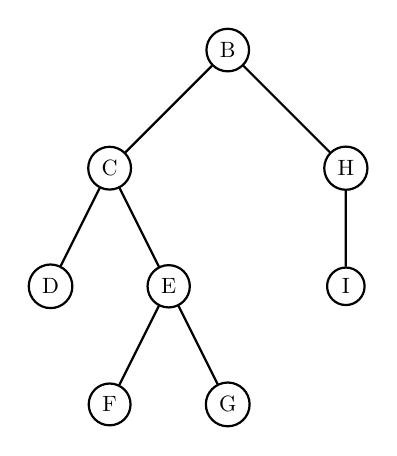
\begin{tikzpicture}[thick,scale=1.0, every node/.style={scale=0.8}]
            \node [circle,draw] {B}
            child {node [circle,draw] {C}
                    child {node [circle,draw] {D}}
                    child {node [circle,draw] {E}
                        child {node [circle,draw] {F}}
                        child {node [circle,draw] {G}}
                    }
            }	
            child [missing] {}
            child {node [circle,draw] {H}
                child {node [circle,draw] {I}}
            };
        \end{tikzpicture}
    \end{center}

    \begin{solution}

        \begin{minipage}{.14\linewidth}
            \begin{tikzpicture}[scale=0.5]
                \cell{}
                \cell{}
                \cell{}
                \cell{E}
            \end{tikzpicture}
        \end{minipage}
        $\to$
        \begin{minipage}{.14\linewidth}
            \begin{tikzpicture}[scale=0.5]
                \cell{}
                \cell{}
                \cell{}
                \cell{}
            \end{tikzpicture}
        \end{minipage}
        $\to$
        \begin{minipage}{.14\linewidth}
            \begin{tikzpicture}[scale=0.5]
                \cell{}
                \cell{C}
                \cell{F}
                \cell{G}
            \end{tikzpicture}
        \end{minipage}
        $\to$
        \begin{minipage}{.14\linewidth}
            \begin{tikzpicture}[scale=0.5]
                \cell{}
                \cell{}
                \cell{F}
                \cell{G}
            \end{tikzpicture}
        \end{minipage}
        $\to$
        \begin{minipage}{.14\linewidth}
            \begin{tikzpicture}[scale=0.5]
                \cell{B}
                \cell{D}
                \cell{F}
                \cell{G}\cellptr{\tiny {stack bottom}}
            \end{tikzpicture}
        \end{minipage}
        $\to$

        \begin{minipage}{.14\linewidth}
            \begin{tikzpicture}[scale=0.5]
                \cell{}
                \cell{D}
                \cell{F}
                \cell{G}
            \end{tikzpicture}
        \end{minipage}
        $\to$
        \begin{minipage}{.14\linewidth}
            \begin{tikzpicture}[scale=0.5]
                \cell{H}
                \cell{D}
                \cell{F}
                \cell{G}
            \end{tikzpicture}
        \end{minipage}
        $\to$
        \begin{minipage}{.14\linewidth}
            \begin{tikzpicture}[scale=0.5]
                \cell{}
                \cell{D}
                \cell{F}
                \cell{G}
            \end{tikzpicture}
        \end{minipage}
        $\to$
        \begin{minipage}{.14\linewidth}
            \begin{tikzpicture}[scale=0.5]
                \cell{I}
                \cell{D}
                \cell{F}
                \cell{G}
            \end{tikzpicture}
        \end{minipage}
        $\to$
        \begin{minipage}{.14\linewidth}
            \begin{tikzpicture}[scale=0.5]
                \cell{}
                \cell{D}
                \cell{F}
                \cell{G} 
            \end{tikzpicture}
        \end{minipage}
        $\to$

        \begin{minipage}{.14\linewidth}
            \begin{tikzpicture}[scale=0.5]
                \cell{}
                \cell{}
                \cell{F}
                \cell{G}
            \end{tikzpicture}
        \end{minipage}
        $\to$
        \begin{minipage}{.14\linewidth}
            \begin{tikzpicture}[scale=0.5]
                \cell{}
                \cell{}
                \cell{}
                \cell{G}
            \end{tikzpicture}
        \end{minipage}
        $\to$
        \begin{minipage}{.14\linewidth}
            \begin{tikzpicture}[scale=0.5]
                \cell{}
                \cell{}
                \cell{}
                \cell{}
            \end{tikzpicture}
        \end{minipage}
        $\to$
        \begin{minipage}{.14\linewidth}
            \begin{tikzpicture}[scale=0.5]
                \cell{}
                \cell{}
                \cell{}
                \cell{}
            \end{tikzpicture}
        \end{minipage}
        $\to$
        \begin{minipage}{.14\linewidth}
            \begin{tikzpicture}[scale=0.5]
                \cell{}
                \cell{}
                \cell{}
                \cell{}
            \end{tikzpicture}
        \end{minipage}

        Traversal Sequence: E, C, B, H, I, D, F, G
    \end{solution}
    
    \newpage
    \part[4] Use queue to run \textbf{Breadth First Traversal} in the tree with root P and you should fill queue step by step and then write down the traversal sequence. 

    \begin{center}
        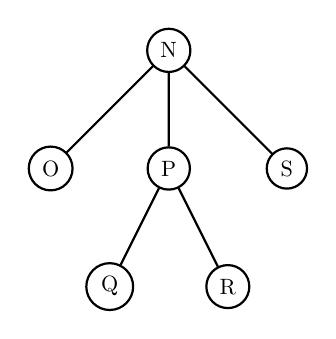
\begin{tikzpicture}
            [thick,scale=1, every node/.style={scale=0.8}]
            \node [circle,draw] {N}
                child {node [circle,draw] {O}}
                child {node [circle,draw] {P}
                    child {node [circle,draw] {Q}}
                    child {node [circle,draw] {R}}	
                }
                child {node [circle,draw] {S}};
        \end{tikzpicture}
    \end{center}
    \begin{solution}\par
        \begin{minipage}{.14\linewidth}
            \begin{tikzpicture}[scale=0.5]
                \cell{}
                \cell{}
                \cell{}
                \cell{P}
            \end{tikzpicture}
        \end{minipage}
        $\to$
        \begin{minipage}{.14\linewidth}
            \begin{tikzpicture}[scale=0.5]
                \cell{}
                \cell{}
                \cell{}
                \cell{}
            \end{tikzpicture}
        \end{minipage}
        $\to$
        \begin{minipage}{.14\linewidth}
            \begin{tikzpicture}[scale=0.5]
                \cell{}
                \cell{R}
                \cell{Q}
                \cell{N}
            \end{tikzpicture}
        \end{minipage}
        $\to$
        \begin{minipage}{.14\linewidth}
            \begin{tikzpicture}[scale=0.5]
                \cell{}
                \cell{}
                \cell{R}
                \cell{Q}
            \end{tikzpicture}
        \end{minipage}
        $\to$
        \begin{minipage}{.14\linewidth}
            \begin{tikzpicture}[scale=0.5]
                \cell{S}
                \cell{O}
                \cell{R}
                \cell{Q}\cellptr{\tiny {queue front}}
            \end{tikzpicture}
        \end{minipage}
        $\to$

        \begin{minipage}{.14\linewidth}
            \begin{tikzpicture}[scale=0.5]
                \cell{}
                \cell{S}
                \cell{O}
                \cell{R}
            \end{tikzpicture}
        \end{minipage}
        $\to$
        \begin{minipage}{.14\linewidth}
            \begin{tikzpicture}[scale=0.5]
                \cell{}
                \cell{}
                \cell{S}
                \cell{O}
            \end{tikzpicture}
        \end{minipage}
        $\to$
        \begin{minipage}{.14\linewidth}
            \begin{tikzpicture}[scale=0.5]
                \cell{}
                \cell{}
                \cell{}
                \cell{S}
            \end{tikzpicture}
        \end{minipage}
        $\to$
        \begin{minipage}{.14\linewidth}
            \begin{tikzpicture}[scale=0.5]
                \cell{}
                \cell{}
                \cell{}
                \cell{}
            \end{tikzpicture}
        \end{minipage}
        $\to$
        \begin{minipage}{.14\linewidth}
            \begin{tikzpicture}[scale=0.5]
                \cell{}
                \cell{}
                \cell{}
                \cell{} 
            \end{tikzpicture}
        \end{minipage}

        Traversal Sequence: P, N, Q, R, O, S
    \end{solution}

\end{parts}